%----------------------------------------------------------------------------------------
%	PACKAGES AND DOCUMENT CONFIGURATIONS
%----------------------------------------------------------------------------------------

\documentclass{article}


\usepackage{graphicx} % Required for the inclusion of images
\graphicspath{{figures/}}
\usepackage{subfigure} % Required for the inclusion of images
\usepackage{natbib} % Required to change bibliography style to APA
\usepackage{amsmath} % Required for some math elements 
\usepackage{listings}
\usepackage{xcolor}
\usepackage{fontspec}
%\usepackage{ctex}
\usepackage{geometry}
%\geometry{a4paper,scale=0.8}
\renewcommand{\contentsname}{\centerline{目录}}
\setmonofont{Consolas}
\lstset{
basicstyle=\ttfamily\footnotesize,%
escapeinside=``,%
keywordstyle=\color{black},%\bfseries, \underbar,%
identifierstyle={},%
tabsize=4,
commentstyle=\color{blue},%
stringstyle=\ttfamily,%
%labelstyle=\tiny,%
extendedchars=false,%
linewidth=\textwidth,%
numbers=left,%
numberstyle=\tiny \color{blue},%
frame=trbl%
}
%点列
%\begin{itemize}
%\item[$\bullet$]Get familiar with Y86 assembly language.
%\end{itemize}

%小标题
%\begin{center}
%{\ttfamily rsum.ys}
%\end{center}
%代码
%\begin{lstlisting}[language={[ANSI]C}]
%\end{lstlisting}
%点列和浮动体图表和ref
%\begin{itemize}
%\item[$\bullet$]{\ttfamily sum.ys} (Figure \ref{Part A: sum.ys})
%\end{itemize}
%\begin{figure}[htbp]
%		\centering
%		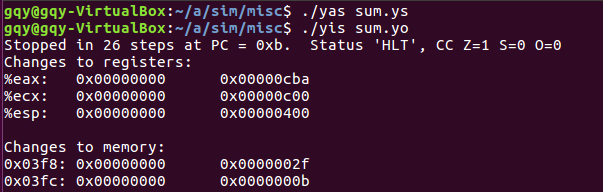
\includegraphics{A_sum}
%		\caption{Part A  {\ttfamily sum.ys}} \label{Part A: sum.ys}
%\end{figure}


%\usepackage{times} % Uncomment to use the Times New Roman font

%----------------------------------------------------------------------------------------
%	DOCUMENT INFORMATION
%----------------------------------------------------------------------------------------


\title{\textbf{Project 2:  Understanding Cache Memories}} % Title

\author{519021910095, Qianyun Guo, guoqianyun@sjtu.edu.cn } % Author name and email

\date{\today} % Date for the report

\begin{document}

\maketitle % Insert the title, author and date

\section{Introduction}

In this project, I had a deep understanding of the working mechanism of cache. In part A, I wrote a cache simulator using C language, which simulates the behavior of a cache memory and records the counts of hit, miss and eviction during the test work. In part B, I tried to optimize a matrix transpose function with the goal of making it cache friendly, which means reduce the miss count during the execution of matrix transpose according to the understanding of cache operation mechanism.

\section{Experiments}

\subsection{Part A}

\subsubsection{Analysis}

This part is about writing a cache simulator using C language. To put it simply, the C program should have the following functions: analyzing the memory trace in the reference trace files as input, maintaining the operation of the cache based on the input, using variables to record the counts of hit, miss, and eviction. The difficult points and code techniques for this part are as follows.\\

\noindent\textbf{Difficult points}
\begin{itemize}
\item[$\bullet$]Analyzing the input from the reference trace files.
\item[$\bullet$]Having a deep understanding of the working mechanism of cache (set-associate).
\item[$\bullet$]Using proper methods to maintaining the operation of the cache.
\item[$\bullet$]The implementation of LRU replacement strategy.
\end{itemize}
\textbf{Code techniques}
\begin{itemize}
\item[$\bullet$]Set the counts of hit, miss and eviction as global static variables for functions to maintain.
\item[$\bullet$]Design a BLOCK struct to simulate cache block with valid-invalid bit, tag information and LRU record.
\item[$\bullet$]Design a CACHE struct to simulate cache with the number of ways per set, number of sets in the cache, the size of each block and a pointer pointed to the cache address.
\item[$\bullet$]Design a function (str\_int) to change the decimal data in a string to an integer.
\item[$\bullet$]Design a function (hex\_dec) to change the hexadecimal data in a string to long type, which is used for analyzing memory address.
\item[$\bullet$]Design a function (parse) to analyze the memory trace in the reference trace files and get the operation type and memory address.
\item[$\bullet$]Design a function (execute) to simulate accessing an address in the cache, with the use of LRU replacement strategy. Pay attention to maintaining hit, miss, and eviction variables.
\item[$\bullet$]In function main(), we first analyze the command to get important parameters for initializing the cache, then open the trace files and simulate cache operation using the above functions.
\item[$\bullet$]LRU replacement strategy implementation. \\
Using the count to record the cumulative memory trace. Each time the program read in a memory trace, update the count. In the function execute(), the count is used to update the LRU record of accessed block. In this case, when cache have to search an eviction, the block that has the minimum LRU record means it is the one the longest not visited, and it would be chosen to be the eviction.
\end{itemize}
To enhance code readability, I wrote necessary comments for critical steps in my codes, please refer to the code section.
 
\subsubsection{Code}
\begin{center}
{\ttfamily csim.c}
\end{center}
\begin{lstlisting}[language={[ANSI]C}]
//Guo Qianyun 519021910095
#include "cachelab.h"
#include <getopt.h>
#include <stdlib.h>
#include <unistd.h>
#include <stdio.h>
#include <string.h>
#define BUFFERSIZE 50
static int hit = 0;		//hit count
static int miss = 0;	//miss count
static int eviction = 0;//eviction count
struct BLOCK {			//cache block
	int valid;			//valid-invalid bit
	long tag;			//tag infomation
	int LRU;			//LRU record
};

struct CACHE {
	int waynum;		//E associativity: num of ways per set
	int setnum;		//2^s num of sets
	int blocksize;	//2^b b: num of block bits
	struct BLOCK **c; 
};
int str_int(char *str);		//change decimal str to int
long hex_dec(char *str);	//change hex str to decimal
//analyze the memory trace and get the operation type and memory address
void parse(char *buffer, char *op, long *add);
//simulate accessing an address in the cache, using LRU
void execute(struct CACHE *cache, long address, int cnt);


int main(int argc, char *argv[])
{
	struct CACHE cache;
	int s, b, S, E, B = 0;
	FILE *fp = NULL;			//for tracefile
	char buffer[BUFFERSIZE];	//for instruction in tracefile
	
	//get S, E, B
	for(int i = 0; i < argc; i++)
	{
		if(argv[i][0] == '-')
		{
			if(argv[i][1] == 's')
			{
				i++;
				s = str_int(argv[i]);
				S = 1 << s;//2^s
			}
			if(argv[i][1] == 'E')
			{
				i++;
				E = str_int(argv[i]);
			}
			if(argv[i][1] == 'b')
			{
				i++;
				b = str_int(argv[i]);
				B = 1 << b;//2^b
			}
			if(argv[i][1] == 't')
			{
				i++;
				if((fp = fopen(argv[i], "r")) == NULL)
				{
					printf("  ERROR: FILE %s OPEN FAILED", argv[i]);
					exit(1);
				}
			}
		}
	}
	if (s <= 0 || E <= 0 || b <= 0)
	{
		printf("  ERROR: INVALID PARAMETER");
		exit(1);
	}
	
	//initialize cache
	cache.waynum = E;
	cache.setnum = S;
	cache.blocksize = B;
	cache.c = (struct BLOCK **) malloc (sizeof(struct BLOCK *) * S);//S sets
	for (int i = 0; i < S; i++)
	{
		// E ways per set
		cache.c[i] = (struct BLOCK *) malloc (sizeof(struct BLOCK) * E);
		//initialize each block
		for(int j = 0; j < E; j++)
		{
			cache.c[i][j].valid = 0;
			cache.c[i][j].tag = 0;
			cache.c[i][j].LRU = 0;
		}
	}
	
	int cnt = 0;
	while(fgets(buffer,sizeof(buffer), fp))	//read in next memory trace
	{
		cnt++;
		char op;
		long address;
		parse(buffer, &op, &address);	//get operation and address
		if(op == 'I') continue;			//skip instruction cache accesses
		execute(&cache, address, cnt);
		if(op == 'M')					//M execute twice
			execute(&cache, address, cnt);
	}
    printSummary(hit, miss, eviction);
    return 0;
}

//change decimal str to int
int str_int(char *str)
{
	int len = strlen(str);
	int res = 0;
	for(int i = 0; i < len; i++)
	{
		res = res * 10 + str[i] - '0';
	}
	return res;
}

//change hex str to decimal
long hex_dec(char *str)
{
	int len = strlen(str);
	long res = 0;
	for(int i = 0; i < len; i++)
	{
		if(str[i] >='0' && str[i] <= '9')
			res = res * 16 + str[i] - '0';
		if(str[i] >='a' && str[i] <= 'f')
			res = res * 16 + str[i] - 'a' + 10;
		if(str[i] >='A' && str[i] <= 'F')
			res = res * 16 + str[i] - 'A' + 10;	
		
	}
	return res;
}

//simulate accessing an address in the cache, using LRU
void execute(struct CACHE *cache, long address, int cnt)
{
	int set_id = (address / cache->blocksize) % (cache->setnum);	//which set
	long tag_num = (address / cache->blocksize) / (cache->setnum);	//tag info
	//search in the set
	int pos = -1;
	for (int i = 0; i < cache -> waynum; i++)
	{
		//found
		if (cache->c[set_id][i].valid == 1 && cache->c[set_id][i].tag == tag_num)
		{
			hit++;
			cache->c[set_id][i].LRU = cnt;	//update LRU record
			return;
		}
		//not found search if empty
		if(cache->c[set_id][i].valid == 0)
			pos = i;
	}
	miss++;
	if(pos >= 0 && pos < cache->waynum)//miss but still have space
	{
		cache->c[set_id][pos].valid = 1;
		cache->c[set_id][pos].tag = tag_num;
		cache->c[set_id][pos].LRU = cnt;	//update LRU record
		return;
	}
	else//evict
	{
		eviction++;
		int min = cache->c[set_id][0].LRU;
		pos = 0;
		for(int i = 1; i < cache->waynum; i++)	//find eviction (minimum LRU)
		{
			if(cache->c[set_id][i].LRU < min)
			{
				min = cache->c[set_id][i].LRU;
				pos = i;
			}
		}
		cache->c[set_id][pos].tag = tag_num;
		cache->c[set_id][pos].LRU = cnt;	//update LRU record
		cache->c[set_id][pos].valid = 1;
	}
	return;
}

//analyze the memory trace and get the operation type and memory address
void parse(char *buffer, char *op, long *address)
{
	char addr[50];
	int i = 0;
	while (buffer[i] == ' ') i++;
	*op=buffer[i];
	i++;
	while (buffer[i] == ' ') i++;
	int j = 0;
	for(; buffer[i] != ',';i++,j++)
	{
		addr[j] = buffer[i];
	}
	addr[j] = 0;
	*address = hex_dec(addr);//change string to long type
}


\end{lstlisting}
\subsubsection{Evaluation}

\begin{itemize}
\item[$\bullet$]Test for {\ttfamily csim.c} (Figure \ref{Part A: csim.c})\\
Test command are as follows.
\begin{lstlisting}[language={[ANSI]C}]
make
./test-csim
\end{lstlisting}
The command tests the correctness of the cache simulator on the reference traces with different cache parameters. As shown in Figure \ref{Part A: csim.c}, the data of my cache simulator is consistent with the data from reference simulator and get full marks in all the 8 test cases.
\end{itemize}
\begin{figure}[htbp]
		\centering
		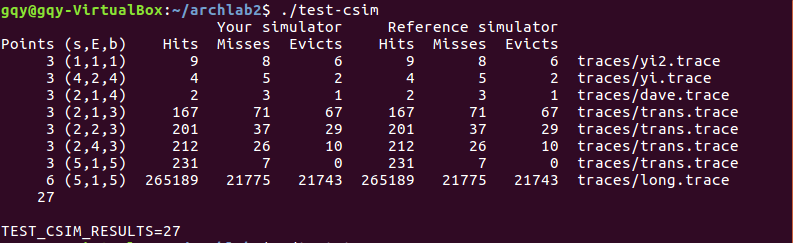
\includegraphics{A}
		\caption{Part A  {\ttfamily csim.c}} \label{Part A: csim.c}
\end{figure}

\subsection{Part B}

\subsubsection{Analysis}

This part is about optimizing a matrix transpose function in order to get better cache performance, that is to say, the function causes as few cache-misses as possible. The tests evaluate 3 different-sized matrices: 32*32, 64*64, 61*67 with cache parameters s = 5, E = 1, b = 5. Before starting, it is important to analyze the cache situation according to different sizes. The difficult points and code techniques as well as thoughts for this part are as follows.\\

\noindent\textbf{Difficult points}
\begin{itemize}
\item[$\bullet$]Analyzing the cache situation for each test size with parameters provided.
\item[$\bullet$]Designing proper method to reduce misses.
\item[$\bullet$]Allocate variables reasonably.
\end{itemize}
\textbf{Code techniques and thoughts (Classified discussion)}
\begin{itemize}
\item[$\bullet$]32*32
\begin{itemize}
\item[$\bullet$]Create 8 temporary variables to help transpose the matrices.
\item[$\bullet$]Block matrix, with each part size 8*8. The reasons why I choose 8*8 are as follows.
\begin{itemize}
\item[$\bullet$]Since the cache parameters s = 5, E = 1, b = 5. The cache has 32 sets and each set has one block. The size of each block is 32 so each block contains 8 integers.
\item[$\bullet$]32*32 matrix, with 32 integers in each line. Since each block contains 8 integers and the cache can contain 32 blocks, the matrix element address is continuous so at most continuous 8 lines in A (8*32 integers in total) can be in the cache at the same time. As shown in Figure \ref{cache situation for 32*32 matrix}.
\begin{figure}[htbp]
		\centering
		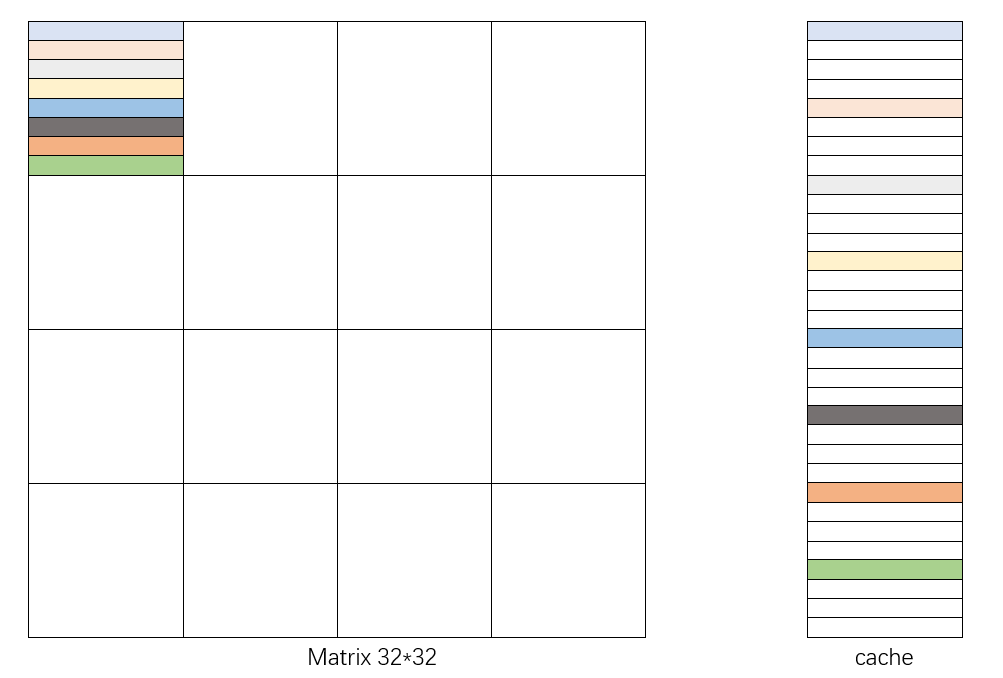
\includegraphics[scale=0.7]{M1}
		\caption{cache situation for 32*32 matrix} \label{cache situation for 32*32 matrix}
\end{figure}
\item[$\bullet$]When executing matrix transpose, the operation in B has the same rules as A. That means, to avoid conflict as much as possible, the size of block matrix is at most 8*8. On the other side, if the size of block size is smaller than 8*8, part of the cache space will be wasted, and part of the data in one cached block will be wasted.
\end{itemize}
\item[$\bullet$]While transpose block matrix, we use the 8 temporary variables instead of using 8 loops like function below for that alternately access matrices A and B may cause unnecessary conflict misses. 
\end{itemize}
\begin{lstlisting}[language={[ANSI]C}]
for (i = 0; i < N; i+=8)
{
   for (j = 0; j < M; j+=8)
    {
        for (a = i; a < i+8; a++) 
        {
            for (b = j; b < j+8; b++)
            {
                B[b][a] = A[a][b];
            }
        }
    }
}
\end{lstlisting}
In this way,  the total miss count is 287.
\item[$\bullet$]64*64
\begin{itemize}
\item[$\bullet$]Create 8 temporary variables to help transpose the matrices.
\item[$\bullet$]Block matrix. Similar to the above analysis, but this time at most continuous 4 lines in A (4*64 integers in total) can be in the cache at the same time. Thus, the first reaction is to choose the size of 4*4. However, the implementation in this way will cause 1699 miss count in total, which has not yet reached the optimization requirements, so further optimization is needed. As shown in Figure \ref{cache situation for 64*64 matrix}.
\begin{figure}[htbp]
		\centering
		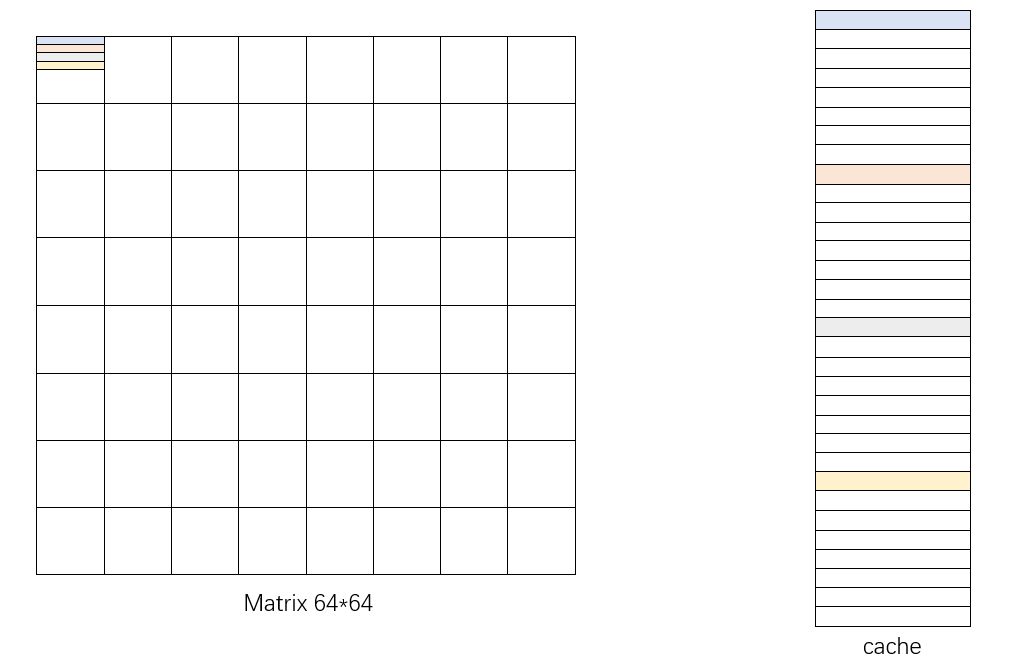
\includegraphics[scale=0.7]{M2}
		\caption{cache situation for 64*64 matrix} \label{cache situation for 64*64 matrix}
\end{figure}
\item[$\bullet$]It can be noticed that when transposing the first 4*4 block matrix, some of the data from A in the cached block has not used yet, and some of the space of B in the cached block has not used either. To make full use of them, we temporarily transpose the unused part of A to unused part of B. In this way, we have to expand the operation range of each loop to 8 * 8.
\item[$\bullet$]The specific steps to transpose 8*8 block matrix are as follows.
\begin{itemize}
\item[$\bullet$]Firstly, transpose the first 4*4 block matrix in A to B (up-left part in A to up-left part in B), and temporarily transpose the up-right 4*4 part in A to the up-right 4*4 part in B for these parts has been cached. As shown in Figure \ref{First Step}.
\begin{figure}[htbp]
		\centering
		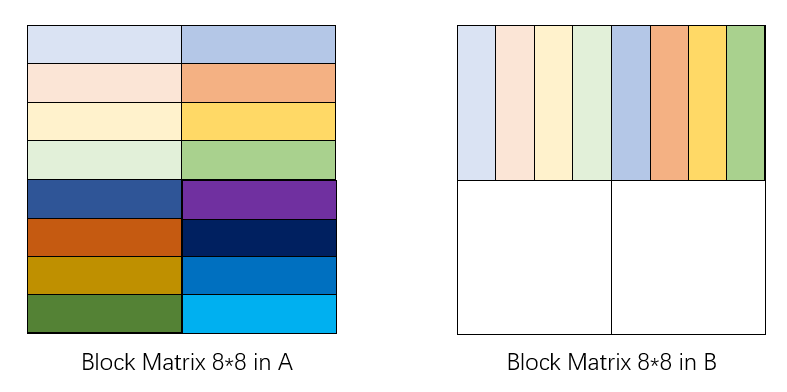
\includegraphics[scale=0.7]{S1}
		\caption{First Step} \label{First Step}
\end{figure}
\item[$\bullet$]Secondly, transpose the down-left 4*4 part in A to the up-right 4*4 part in B and move the temporary data in the up-right 4*4 part in B to the down-left 4*4 part in B. We have to first use 8 temporary variables to record the data for it may be covered during execution. As shown in Figure \ref{Second Step}.
\begin{figure}[htbp]
		\centering
		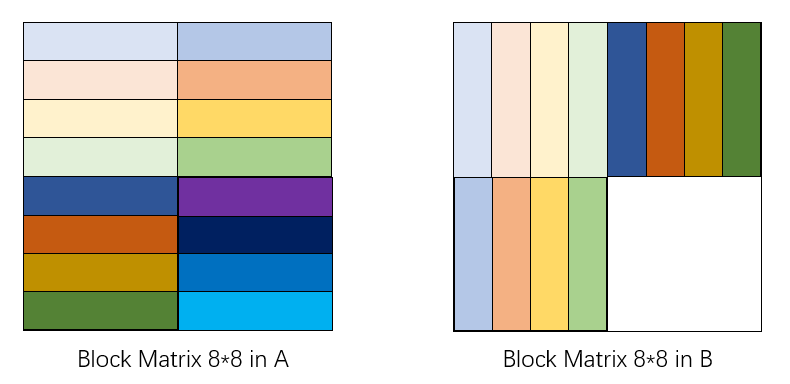
\includegraphics[scale=0.7]{S2}
		\caption{Second Step} \label{Second Step}
\end{figure}
\item[$\bullet$]Thirdly, transpose the down-right 4*4 part in A to the down-right 4*4 part in B. As shown in Figure \ref{Third Step}.
\begin{figure}[htbp]
		\centering
		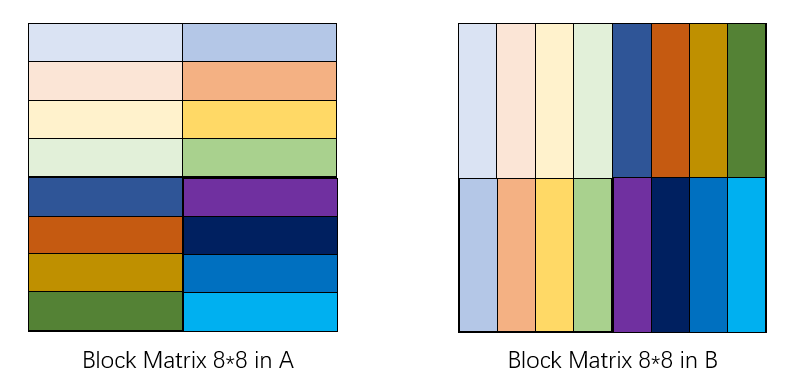
\includegraphics[scale=0.7]{S3}
		\caption{Third Step} \label{Third Step}
\end{figure}
\end{itemize}
\end{itemize}
In this way,  the total miss count is 1179.
\item[$\bullet$]61*67
\begin{itemize}
\item[$\bullet$]We still choose to operate on block matrix, but since M is not equal to N, we can’t use fixed 8 variables as before so we chose to use loops. 
\item[$\bullet$]First, I tried 8*8 block matrix and the miss count reached 2118, which has not yet reached the optimization requirements.
\item[$\bullet$]By accident, I tired 16*16 block matrix and the miss count reached 1992, which has reached the optimization requirements.
\item[$\bullet$]Noticed that the miss count may have correlation to the size of block matrix size. I defined PARTSIZE and change it to test the correlation. The results are shown in the bellow Table \ref{the correlation between PARTSIZE and MISS}
\begin{table}[htbp]
\centering
\caption{the correlation between PARTSIZE and MISS}\label{the correlation between PARTSIZE and MISS}%标题
\begin{tabular}{|c | c| c| c| c| c| c| c| c | p{1.5cm}|}
		%左对齐 居中对齐 右对齐 |产生竖线 ||双竖线 
		%p{}指定宽度,内容超过宽度时自动换行
		\hline%产生表格横线
		PARTSIZE & 4 & 8 & 12 & 16 & 17 & 18 & 19 & 20\\% &表示不同列
		\hline 
		MISS & 2425 & 2118 & 2057 & 1992 & 1950 & 1961 & 1979 & 2002  \\
		\hline
\end{tabular}
\end{table}
\item[$\bullet$]We can see the correlation between miss count and PARTSIZE is a U shape, and when PARTSIZE is 17, we get the lowest point. So finally the PARTSIZE is set to 17.
\end{itemize}
\end{itemize}
To enhance code readability, I wrote necessary comments for critical steps in my codes, please refer to the code section.
\newpage
\subsubsection{Code}
\begin{center}
{\ttfamily trans.c}
\end{center}
\begin{lstlisting}[language={[ANSI]C}]
//Guo Qianyun 519021910095
/* 
 * trans.c - Matrix transpose B = A^T
 *
 * Each transpose function must have a prototype of the form:
 * void trans(int M, int N, int A[N][M], int B[M][N]);
 *
 * A transpose function is evaluated by counting the number of misses
 * on a 1KB direct mapped cache with a block size of 32 bytes.
 */ 
#include <stdio.h>
#include "cachelab.h"
#define PARTSIZE 17
int is_transpose(int M, int N, int A[N][M], int B[M][N]);

/* 
 * transpose_submit - This is the solution transpose function that you
 *     will be graded on for Part B of the assignment. Do not change
 *     the description string "Transpose submission", as the driver
 *     searches for that string to identify the transpose function to
 *     be graded. 
 */
char transpose_submit_desc[] = "Transpose submission";
void transpose_submit(int M, int N, int A[N][M], int B[M][N])
{
	if(M == 32 && N == 32)
	{
		int t0, t1, t2, t3, t4, t5, t6, t7;
		for(int i = 0; i < N; i += 8)
		{
			for(int j = 0; j < M; j +=8)
			{
				for(int a = i; a < i+8; a++)
				{
					int b = j;
					// 8 integer from a line in A
					t0 = A[a][b];
					t1 = A[a][b+1];
					t2 = A[a][b+2];
					t3 = A[a][b+3];
					t4 = A[a][b+4];
					t5 = A[a][b+5];
					t6 = A[a][b+6];
					t7 = A[a][b+7];
					//put to B
					B[b][a] = t0;
					B[b+1][a] = t1;
					B[b+2][a] = t2;
					B[b+3][a] = t3;
					B[b+4][a] = t4;
					B[b+5][a] = t5;
					B[b+6][a] = t6;
					B[b+7][a] = t7;
				}
			}	
		}
	}
	else if(M == 64 && N == 64)
	{
		int t0, t1, t2, t3, t4, t5, t6, t7;
		for(int i = 0; i < N; i += 8)
		{
			for(int j = 0; j < M; j +=8)
			{
				for(int a = i; a < i+4; a++)
				{
					int b = j;
					
					t0 = A[a][b];
					t1 = A[a][b+1];
					t2 = A[a][b+2];
					t3 = A[a][b+3];
					t4 = A[a][b+4];
					t5 = A[a][b+5];
					t6 = A[a][b+6];
					t7 = A[a][b+7];
					
					//up_left part of A to up_left part of B
					B[b][a] = t0;
					B[b+1][a] = t1;
					B[b+2][a] = t2;
					B[b+3][a] = t3;
					
					//temporarily up_right part of A to up_right part of B
					B[b][a+4] = t4;
					B[b+1][a+4] = t5;
					B[b+2][a+4] = t6;
					B[b+3][a+4] = t7;
				}
				for(int b = j; b < j+4; b++)
				{
					int a = i;
					t0 = A[a+4][b];
					t1 = A[a+5][b];
					t2 = A[a+6][b];
					t3 = A[a+7][b];
					
					t4 = B[b][a+4];
					t5 = B[b][a+5];
					t6 = B[b][a+6];
					t7 = B[b][a+7];
					
					//down_left part of A to up_right part of B
					B[b][a+4] = t0;
					B[b][a+5] = t1;
					B[b][a+6] = t2;
					B[b][a+7] = t3;
					
					//the temporary up_right part of B move to down_left part of B
					B[b+4][a] = t4;
					B[b+4][a+1] = t5;
					B[b+4][a+2] = t6;
					B[b+4][a+3] = t7;
				}
				for(int a = i+4; a<i+8; a++)
				{
					int b = j+4;
					t0 = A[a][b];
					t1 = A[a][b+1];
					t2 = A[a][b+2];
					t3 = A[a][b+3];
					
					//down_right part of A to down_right part of B
					B[b][a] = t0;
					B[b+1][a] = t1;
					B[b+2][a] = t2;
					B[b+3][a] = t3;
				}
			}
		}
	}
	else if(M == 61 && N == 67)
	{
		for(int i = 0; i < N; i+=PARTSIZE)
		{
			for(int j = 0; j < M; j+=PARTSIZE)
			{
				for(int a = i; a < i+PARTSIZE && a < N; a++)
				{
					for(int b = j; b < j+PARTSIZE && b < M; b++)
					{
						B[b][a] = A[a][b];
					}
				}
			}
		}
	}
	else
	{
	    int i, j, tmp;
		for (i = 0; i < N; i++) {
			for (j = 0; j < M; j++) {
				tmp = A[i][j];
				B[j][i] = tmp;
			}
		}   
	}
}

/* 
 * You can define additional transpose functions below. We've defined
 * a simple one below to help you get started. 
 */ 

/* 
 * trans - A simple baseline transpose function, not optimized for the cache.
 */
char trans_desc[] = "Simple row-wise scan transpose";
void trans(int M, int N, int A[N][M], int B[M][N])
{
    int i, j, tmp;

    for (i = 0; i < N; i++) {
        for (j = 0; j < M; j++) {
            tmp = A[i][j];
            B[j][i] = tmp;
        }
    }    

}

/*
 * registerFunctions - This function registers your transpose
 *     functions with the driver.  At runtime, the driver will
 *     evaluate each of the registered functions and summarize their
 *     performance. This is a handy way to experiment with different
 *     transpose strategies.
 */
void registerFunctions()
{
    /* Register your solution function */
    registerTransFunction(transpose_submit, transpose_submit_desc); 

    /* Register any additional transpose functions */
    registerTransFunction(trans, trans_desc); 

}

/* 
 * is_transpose - This helper function checks if B is the transpose of
 *     A. You can check the correctness of your transpose by calling
 *     it before returning from the transpose function.
 */
int is_transpose(int M, int N, int A[N][M], int B[M][N])
{
    int i, j;

    for (i = 0; i < N; i++) {
        for (j = 0; j < M; ++j) {
            if (A[i][j] != B[j][i]) {
                return 0;
            }
        }
    }
    return 1;
}

\end{lstlisting}
\subsubsection{Evaluation}
Test command are as follows.
\begin{lstlisting}[language={[ANSI]C}]
make
./test-trans -M 32 -N 32
./test-trans -M 64 -N 64
./test-trans -M 61 -N 67
\end{lstlisting}
\begin{figure}[htbp]
		\centering
		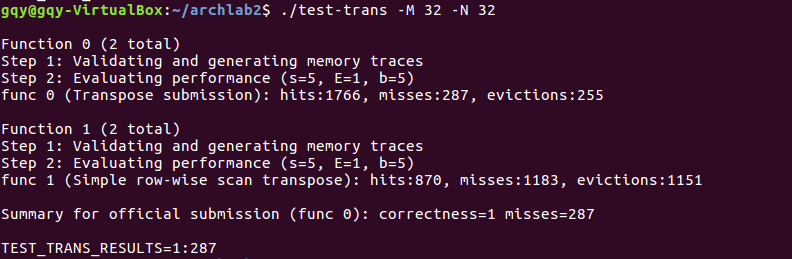
\includegraphics{B1}
		\caption{Part B: M=32, N=32} \label{Part B: M=32, N=32}
\end{figure}
\begin{figure}[htbp]
		\centering
		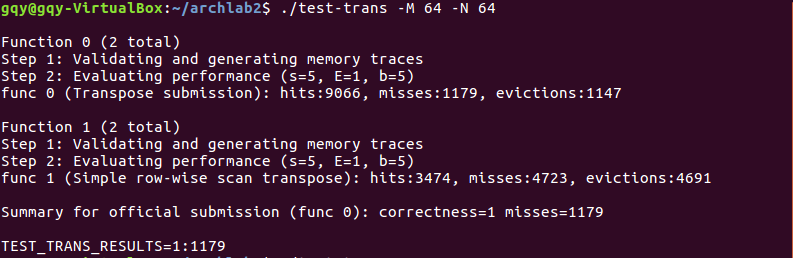
\includegraphics{B2}
		\caption{Part B: M=64, N=64} \label{Part B: M=64, N=64}
\end{figure}
\begin{figure}[htbp]
		\centering
		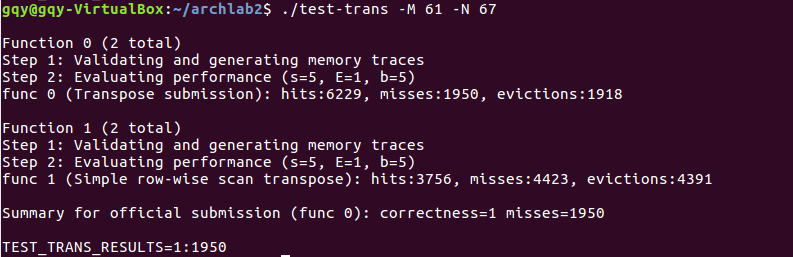
\includegraphics{B3}
		\caption{Part B: M=61, N=67} \label{Part B: M=61, N=67}
\end{figure}
\begin{itemize}
\item[$\bullet$]Test for M=32 and N=32 (Figure \ref{Part B: M=32, N=32})
\item[$\bullet$]Test for M=64 and N=64 (Figure \ref{Part B: M=64, N=64})
\item[$\bullet$]Test for M=61 and N=67 (Figure \ref{Part B: M=61, N=67})
\end{itemize}
The command tests the count of miss of each type of matrix. The count of miss for M=32 and N=32 is 287,  the count of miss for M=64 and N=64 is 1179, the count of miss for M=61 and N=67 is 1950, which all  reached the optimization requirements.
\section{Conclusion}

\subsection{Problems}

\begin{itemize}
\item[$\bullet$]Have a thorough understanding of the mechanism of cache operation. Writing a cache simulator entails a good grasp of the cache mechanism. Since the csim.c is almost empty, we have to write from scratch. At first, I had no clue about where to start, so I chose to review the content of the classes about cache and then figure out the way.
\item[$\bullet$]Figure out implementation method for cache simulation and LRU replacement strategy. To simulate the cache properly we have to create proper functions and structs. Fortunately, I have tried to write a memory simulator with TLB and page table in the operating system class and this part is similar to that, so it can be solved after careful thoughts.
\item[$\bullet$]Figure out further optimization method for 64*64 matrix transpose. When noticing that 4*4 block matrix method is not enough for the optimization requirements, I was stuck in a bottleneck. After an efficient discussion with classmates and a deep personal thought, the further optimization method was figured out finally.
\end{itemize}
\subsection{Achievements}
\begin{itemize}
\item[$\bullet$]In Part A, I successfully wrote a cache simulator which runs correctly with right record of hit count, miss count and eviction count, using LRU replacement strategy.
\item[$\bullet$]In Part B, I carefully analyzed the cache situation under different matrix sizes and optimizing the function step by step. Especially in the optimization step for 64*64 matrix, a little more complex but Intuitive approach was figured out and meet the requirements successfully. In the optimization for 61*67 matrix, I found the best parameter for the block matrix by several testing. Besides, all the optimization steps and my thoughts are illustrated in detail with necessary figures in the analysis part.
\item[$\bullet$]To take care of the readability of the codes, I added detailed comments in each critical step.
\item[$\bullet$]In brief, the project helped me have a better understanding of the cache performance. It provided me with an opportunity to apply theoretical knowledge to practice, which both enhanced my grasp of the knowledge and strengthened my coding ability. By the way, completing the whole project on my own gives me a great sense of achievement.
\end{itemize}
Finally, I would like to appreciate Miss Shen and teaching assistants for their careful guidance and support, from which I have benefited a lot.



%----------------------------------------------------------------------------------------


\end{document}